\section{Resultados del estado actual de los recintos}
A continuación se muestran los resultados de las mediciones y parámetros más específicos del ruido de fondo y tiempo de reverberación, como curvas NC y NR, claridad ($C_{50speech}$, $C_{80}$) y definición $D_{50}$.
\subsection{Ruido de fondo}
En las figuras \ref{fig: Curvas NC sala 1}, \ref{fig: Curvas NC sala 2} y \ref{fig: Curvas NC sala de ensayo}, se pueden observar los valores obtenidos del ruido de fondo en bandas de octava con su respectiva curva NC más cercana.
    \begin{figure}[H]
        \centering
        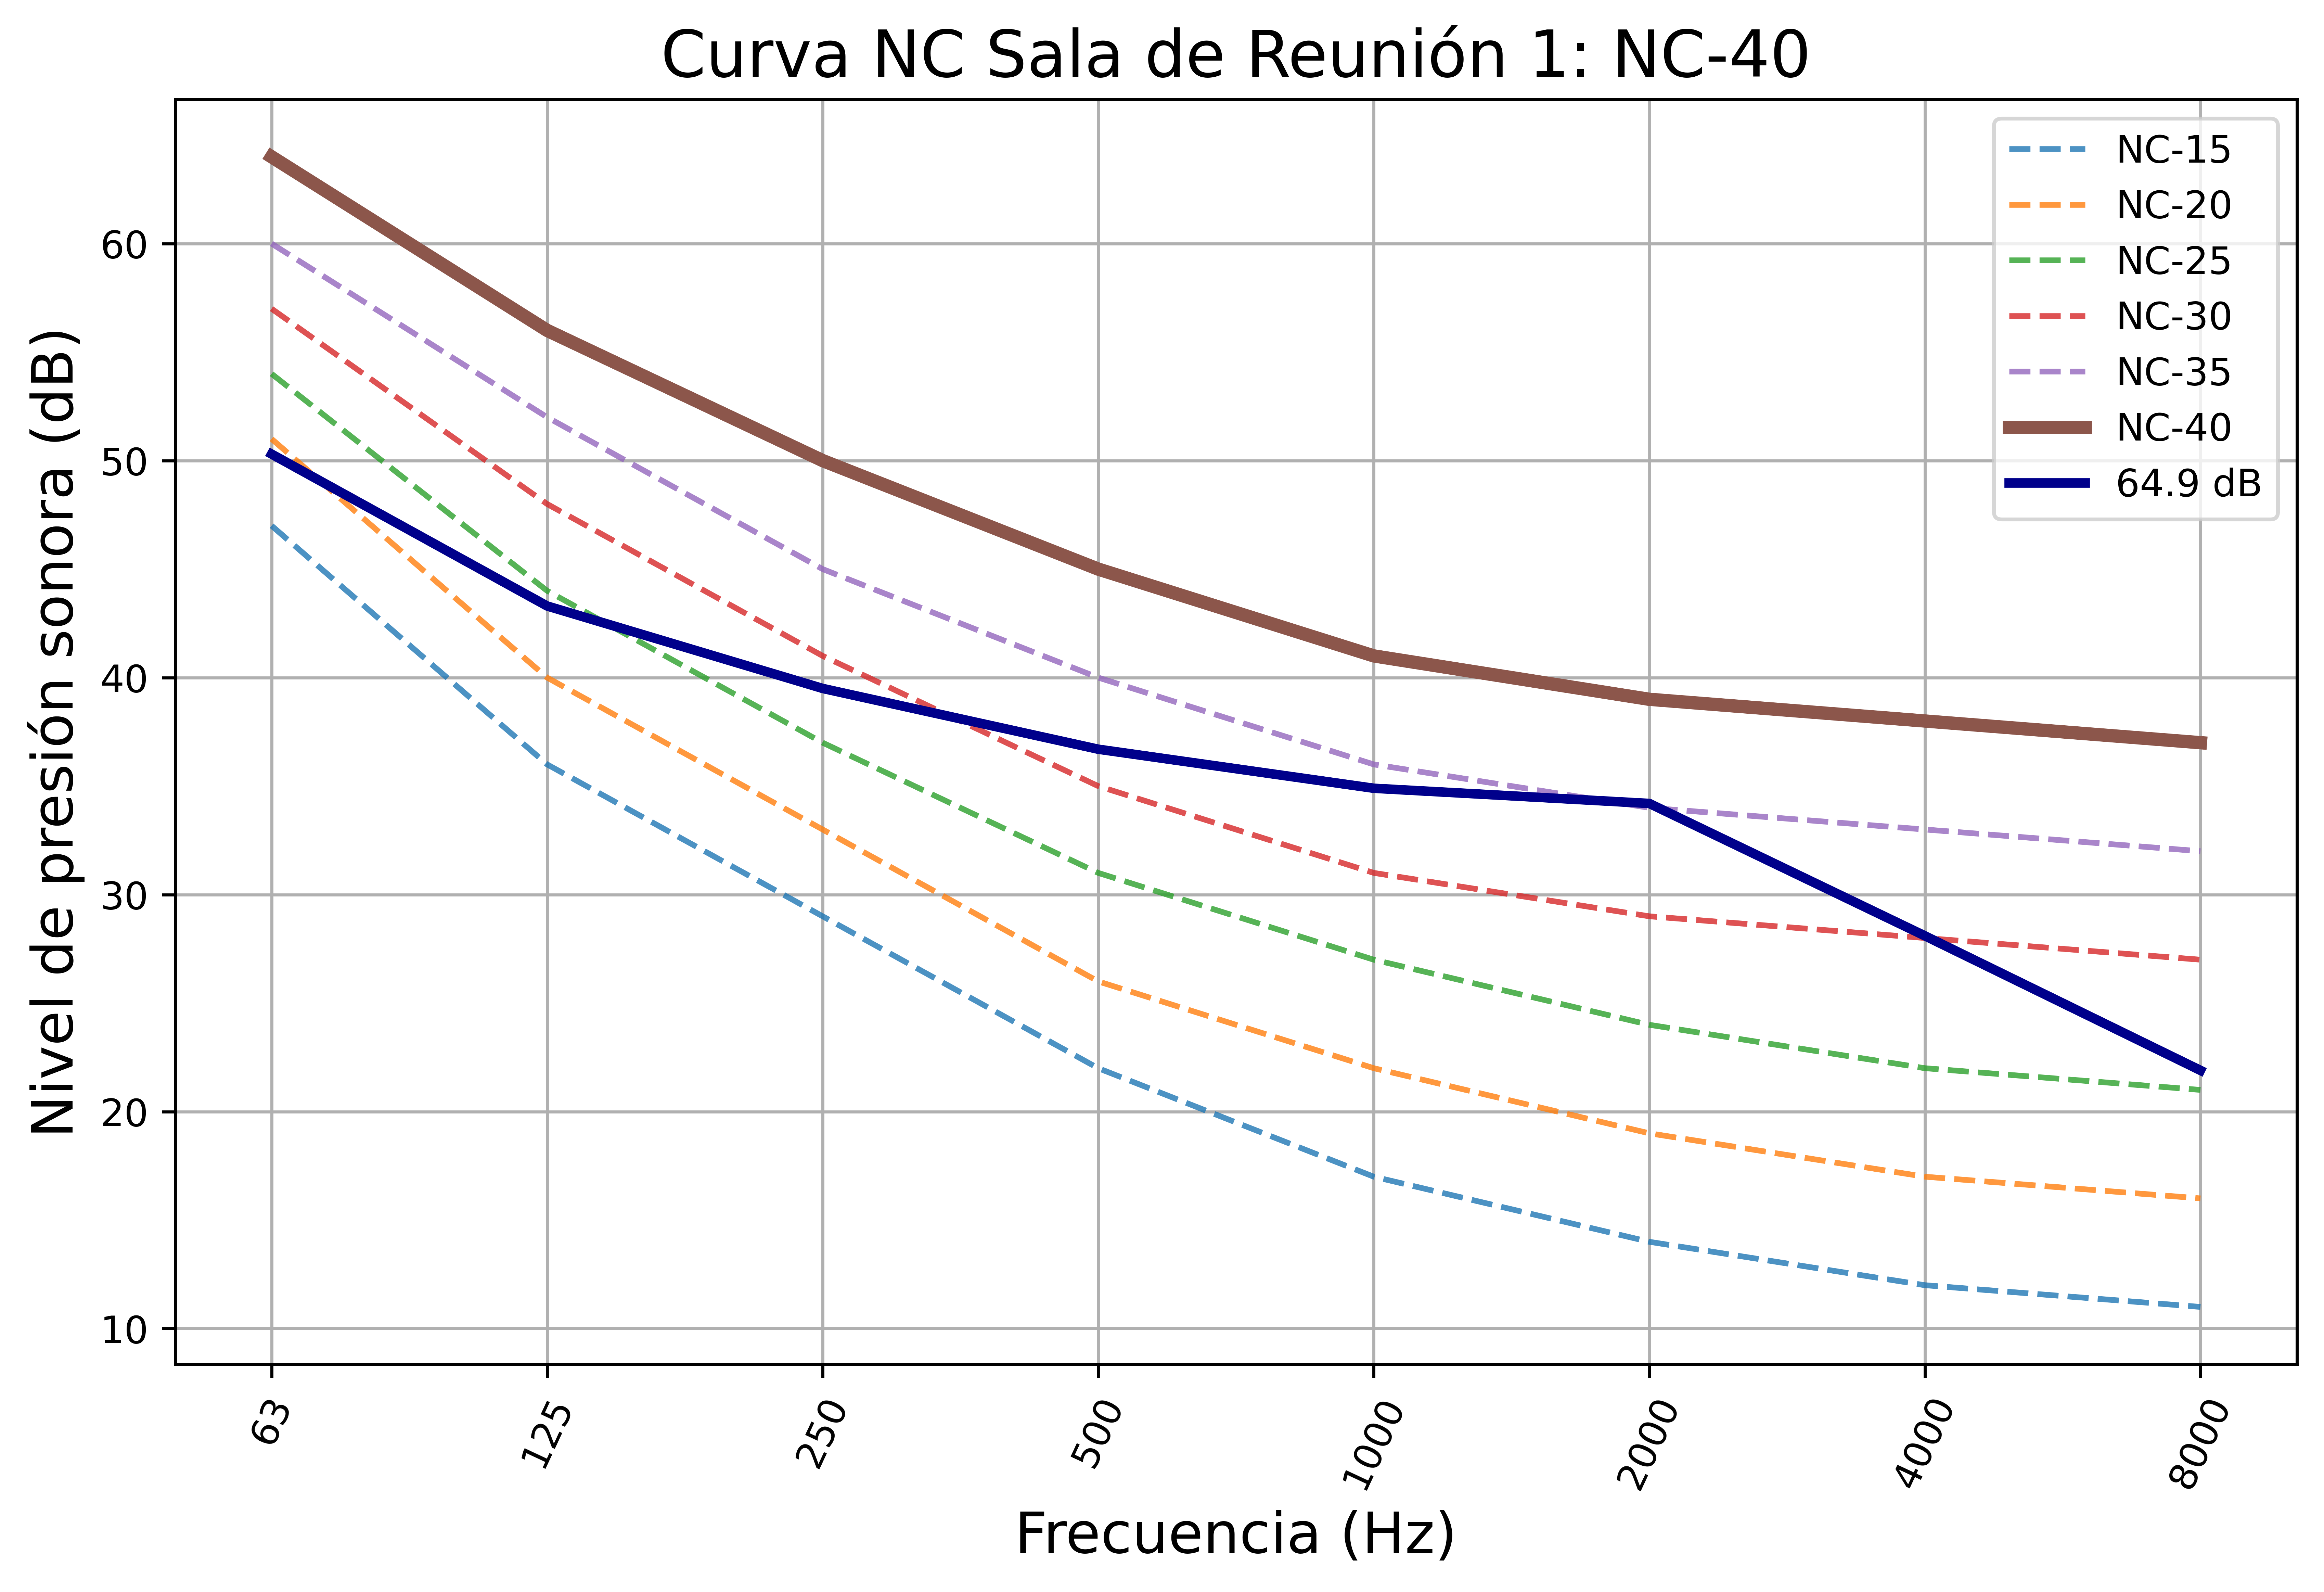
\includegraphics[width=10cm]{Imagenes/Resultados/Curvas NC-NR/NC reunion 1.png}
        \caption{Curvas NC sala de reunión 1}
        \label{fig: Curvas NC sala 1}
    \end{figure}

    \begin{figure}[H]
        \centering
        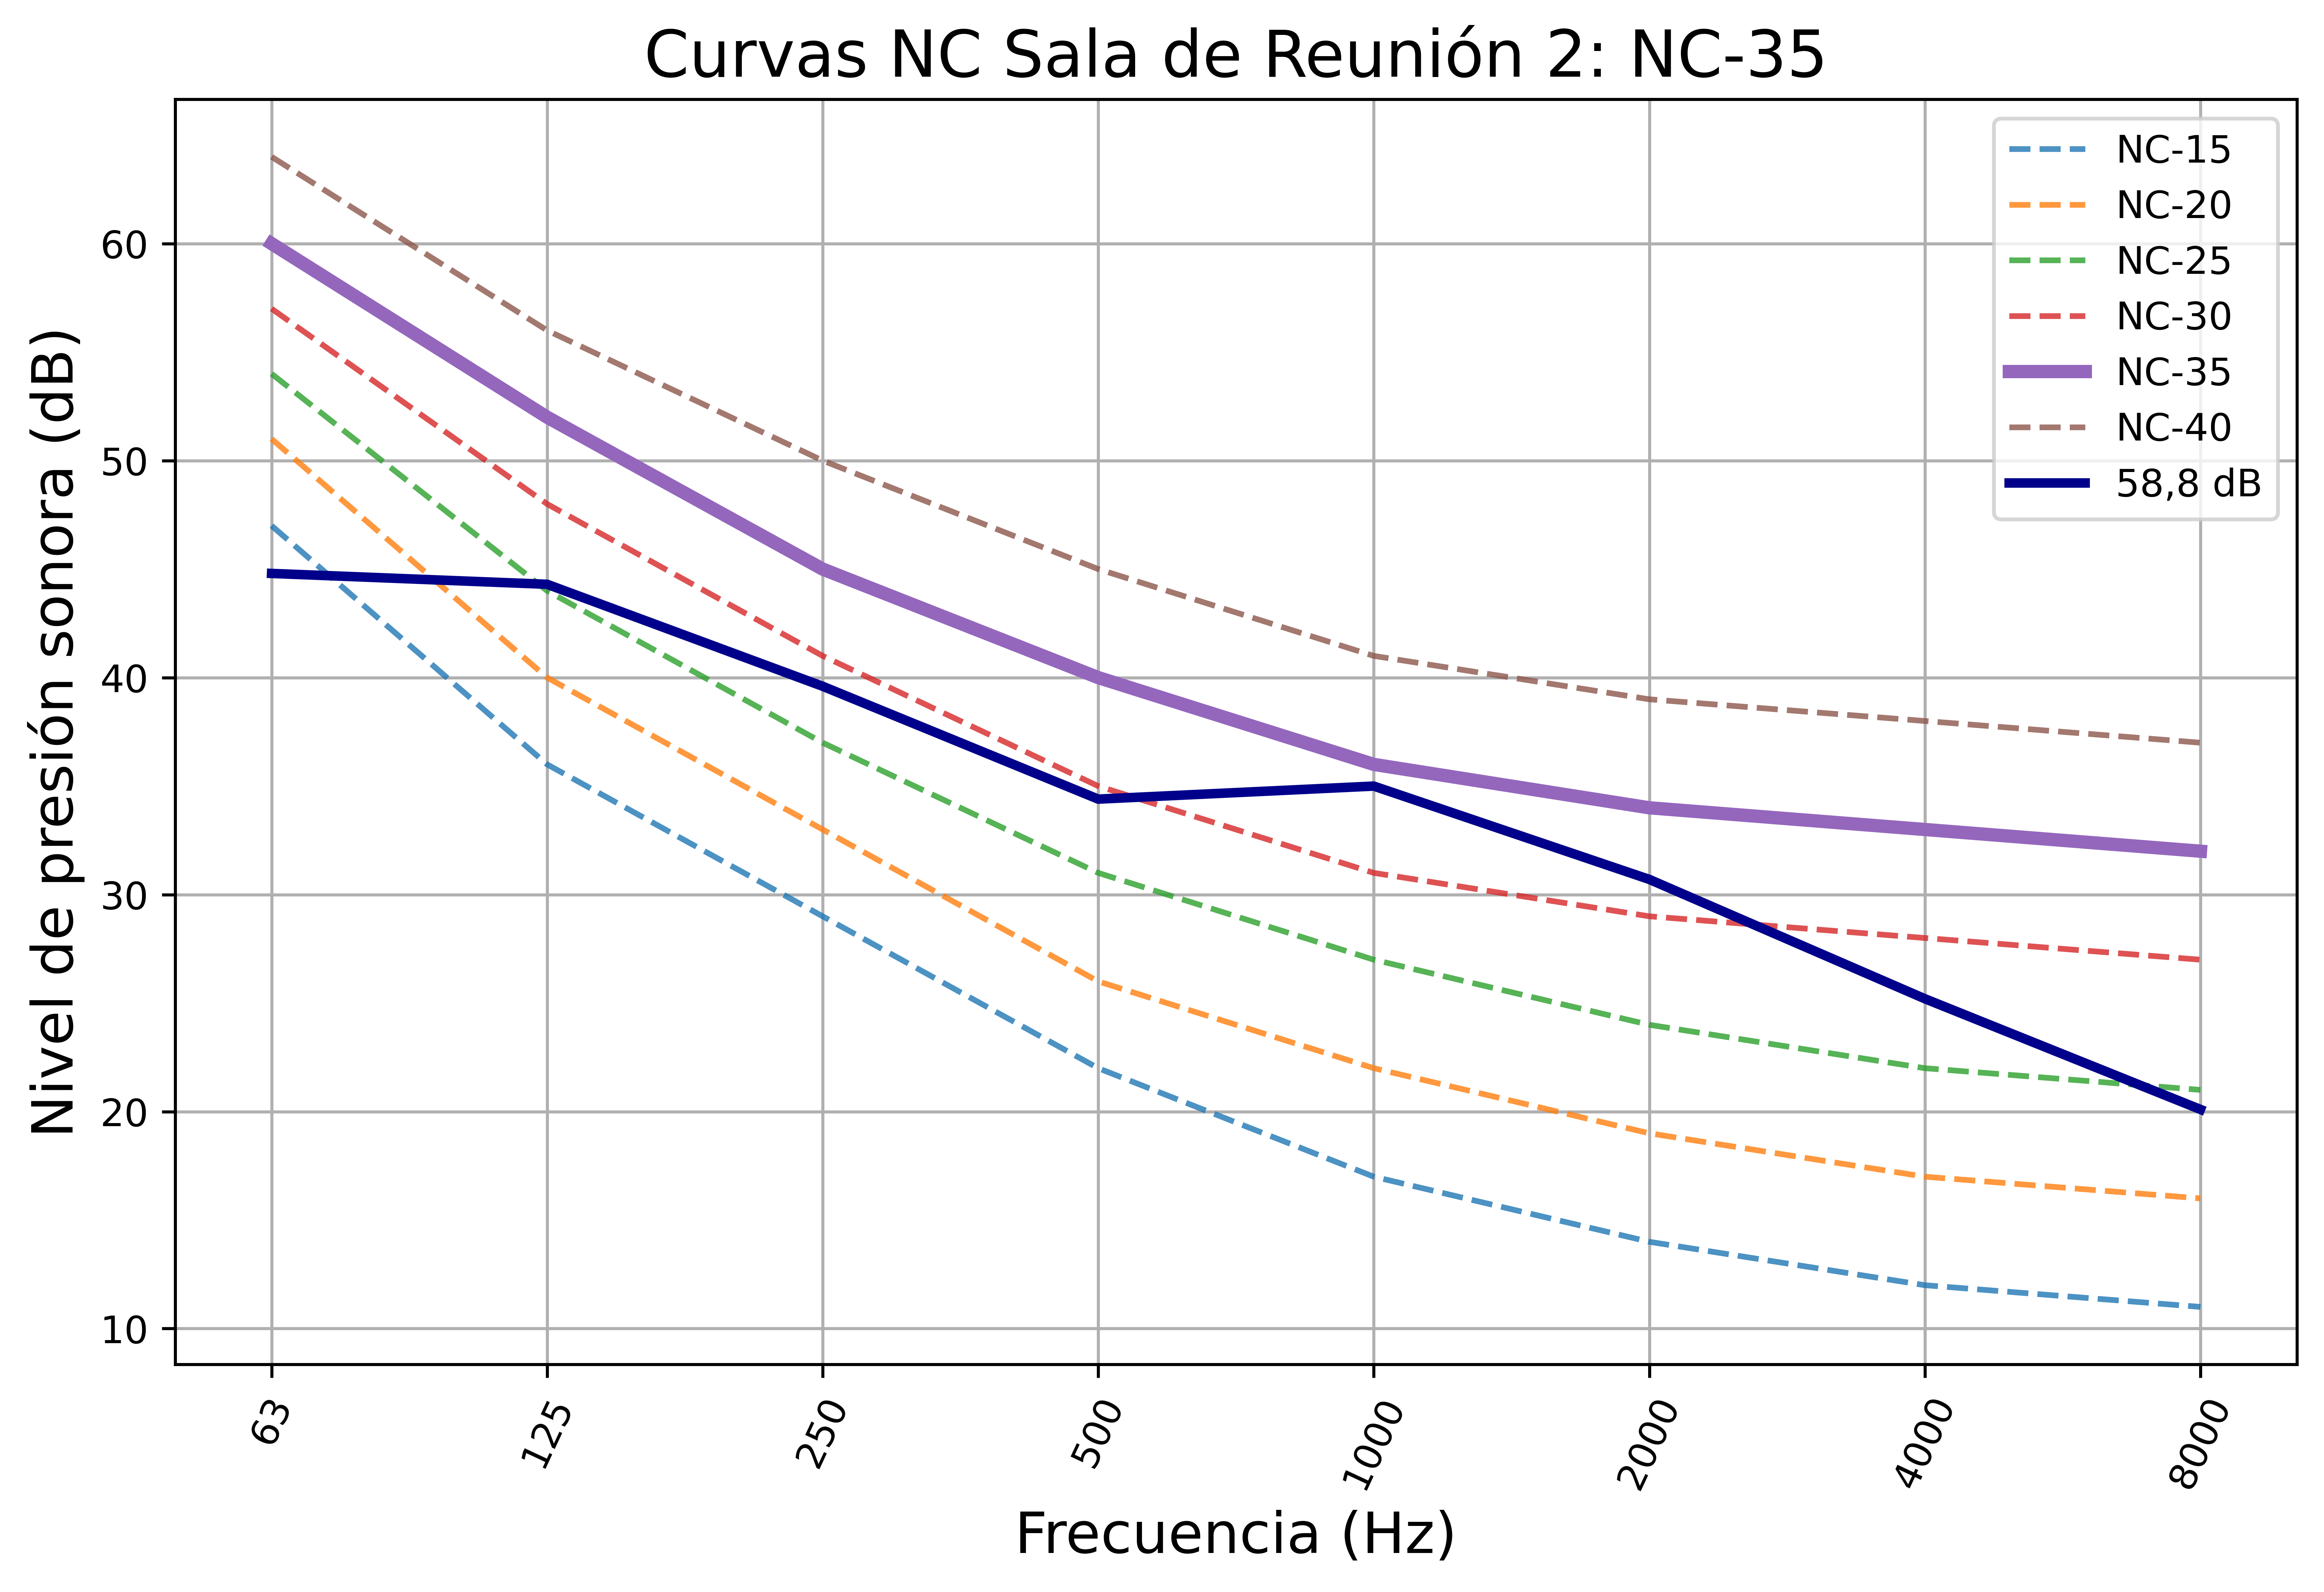
\includegraphics[width=10cm]{Imagenes/Resultados/Curvas NC-NR/NC reunion 2.png}
        \caption{Curvas NC sala de reunión 2}
        \label{fig: Curvas NC sala 2}
    \end{figure}

    \begin{figure}[H]
        \centering
        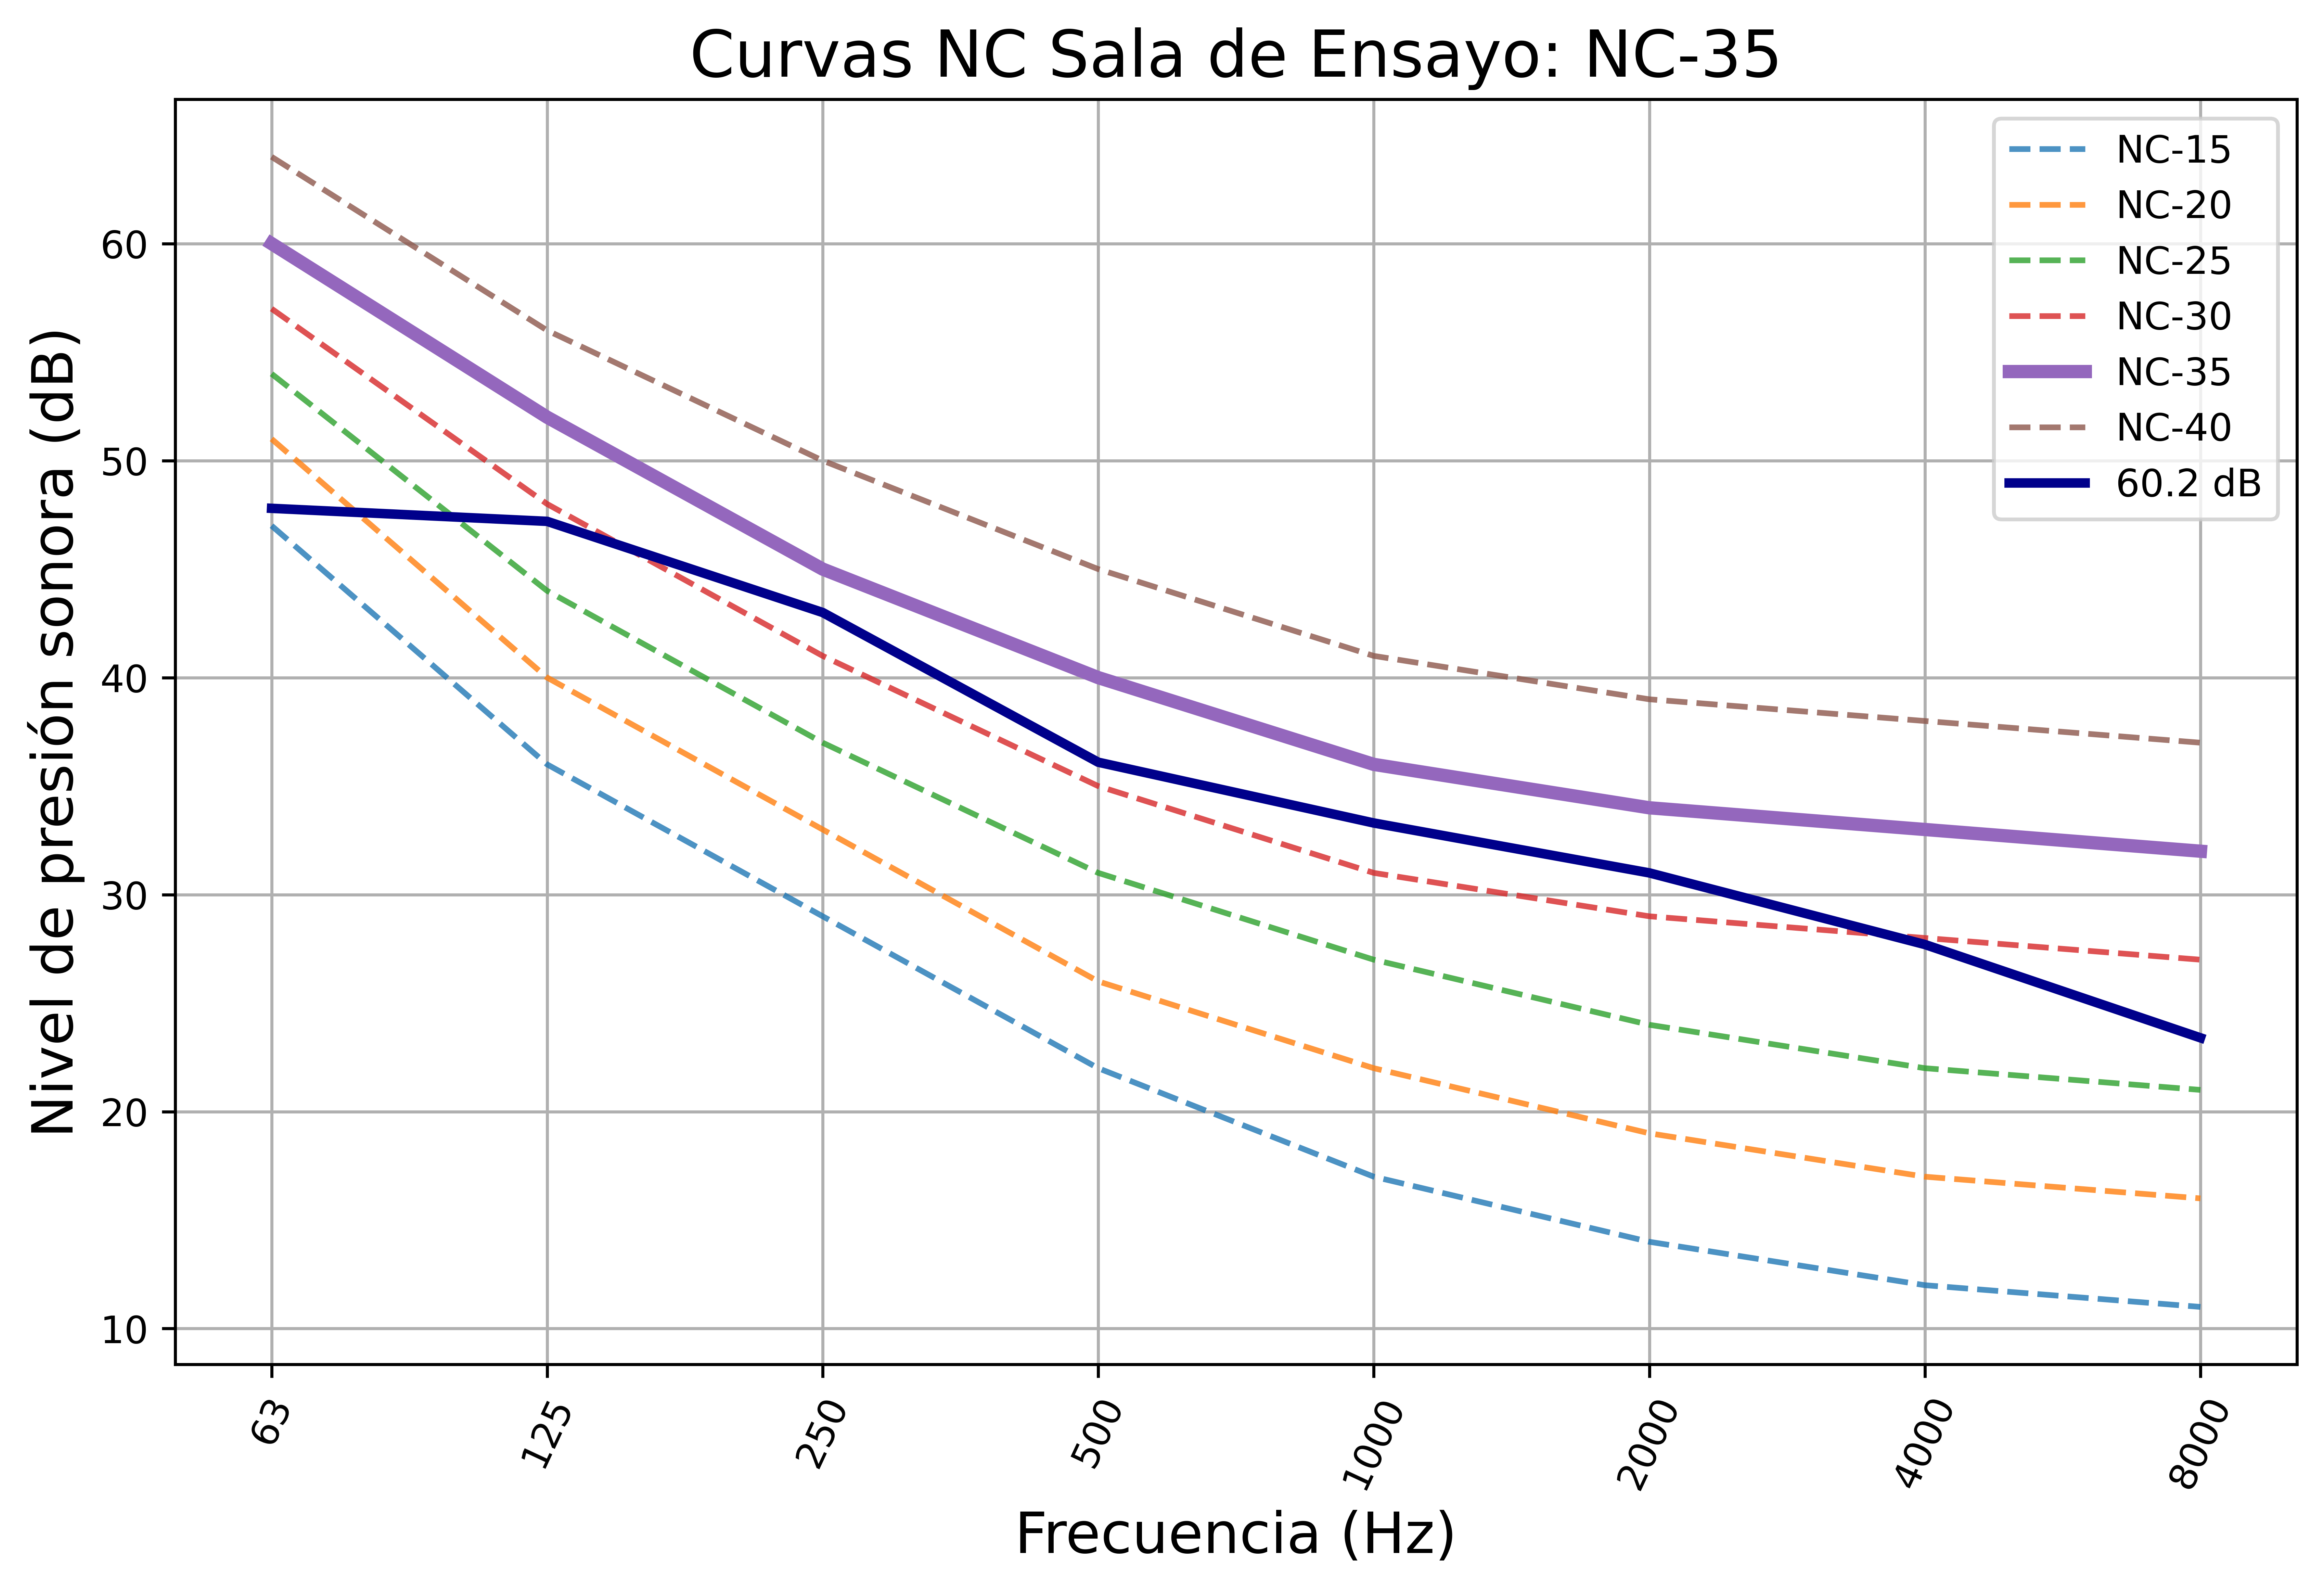
\includegraphics[width=10cm]{Imagenes/Resultados/Curvas NC-NR/NC ensayo.png}
        \caption{Curvas NC sala de ensayo}
        \label{fig: Curvas NC sala de ensayo}
    \end{figure}

Según las recomendaciones mencionadas en la sección \ref{secc: Recomendaciones} se puede determinar que los valores de ruido de fondo como se muestran en la tabla \ref{tab: cumplimiento de Rdf} no cumplen para todas las salas.

\begin{table}[H]
    \centering
    \begin{tabular}{|l|c|c|c|}
    \hline
    \textbf{Salones}  & \textbf{\begin{tabular}[c]{@{}c@{}}Curva NC\\  recomendada\end{tabular}} & \textbf{\begin{tabular}[c]{@{}c@{}}Curva NC\\  medida\end{tabular}} & \textbf{Estado} \\ \hline
    Sala de reunión 1 & $25$ - $30$ & $40$ & \textcolor{red}{No cumple}\\ \hline
    Sala de reunión 2 & $25$ - $30$ & $35$ & \textcolor{red}{No cumple}\\ \hline
    Sala de ensayo    & $20$ - $25$ & $35$ & \textcolor{red}{No cumple} \\ \hline
    \end{tabular}
    \caption{Estado de parámetros de ruido de fondo por sala}
    \label{tab: cumplimiento de Rdf}
    \end{table}

\subsection{Tiempo de reverberación}
\subsubsection{Salas de reunión}
A partir del tiempo de reverberación medido (ver anexo \ref{subseccc: mediciones tiempo de reverberación}), se obtienen los gráficos de tiempo de reverberación descritos en la norma DIN$18041$ para las salas de reunión.
    \begin{figure}[H]
        \centering
        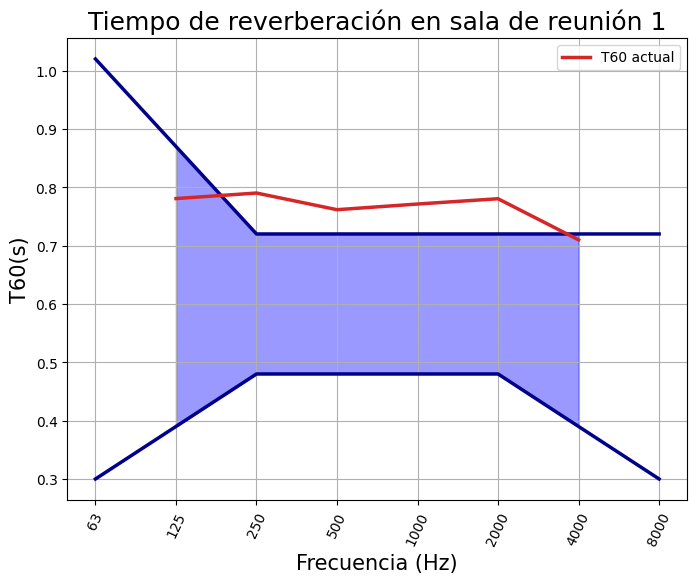
\includegraphics[width=10cm]{Imagenes/DIN/DIN sala reunion 1 actual.png}
        \caption{Tiempo de reverberación Sala de reunión 1}
        \label{fig:Ttarget sala de reunion 1}
    \end{figure}

    \begin{figure}[H]
        \centering
        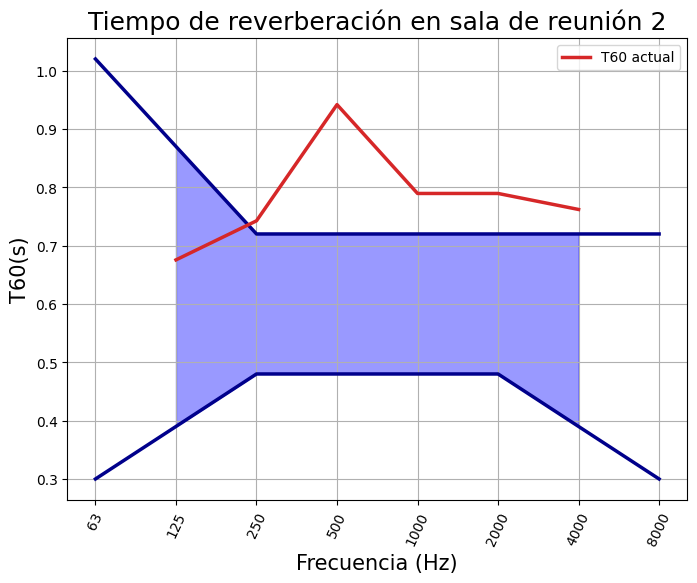
\includegraphics[width=10cm]{Imagenes/DIN/DIN sala reunion 2 actual.png}
        \caption{Tiempo de reverberación Sala de reunión 2}
        \label{fig:Ttarget sala de reunion 2}
    \end{figure}
A continuación se muestra una tabla con los valores obtenidos a partir de las mediciones realizadas. Los gráficos más detallados se encuentran en el anexo.
    %insertar cual anexo
    \begin{table}[H]
        \centering
        \begin{tabular}{|l|c|c|c|}
        \hline
          \textbf{Parámetro}  & \textbf{Recomendación} & \textbf{Sala de reunión $1$} & \textbf{Sala de reunión $2$}\\ \hline
          $T_{target} (s)$    & $0.6$ & \textcolor{red}{No cumple} & \textcolor{red}{No cumple}\\ \hline
          $C_{50speech}$      & $C_{50speech}>0$ & \textcolor{teal}{$1.79$} & \textcolor{teal}{$0.89$} \\ \hline
          STI & STI $> 0.45$  & \textcolor{teal}{$0.66$} & \textcolor{teal}{$0.64$}\\\hline
        \end{tabular}
        \caption{Parámetros acústicos de las salas de reunión}
        \label{tab: cumplimiento parametros RT salas de reuniones}
    \end{table}
\subsubsection{Sala de ensayo}
    Para la sala de ensayo, se determinaron parámetros a partir del tiempo de reverberación, parámetros que se analizaron su cumplimiento con recomendaciones mencionadas en la sección \ref{secc: Recomendaciones}.
    Se obtuvo el siguiente gráfico de definición $D_{50}$:
    \begin{figure}[H]
        \centering
        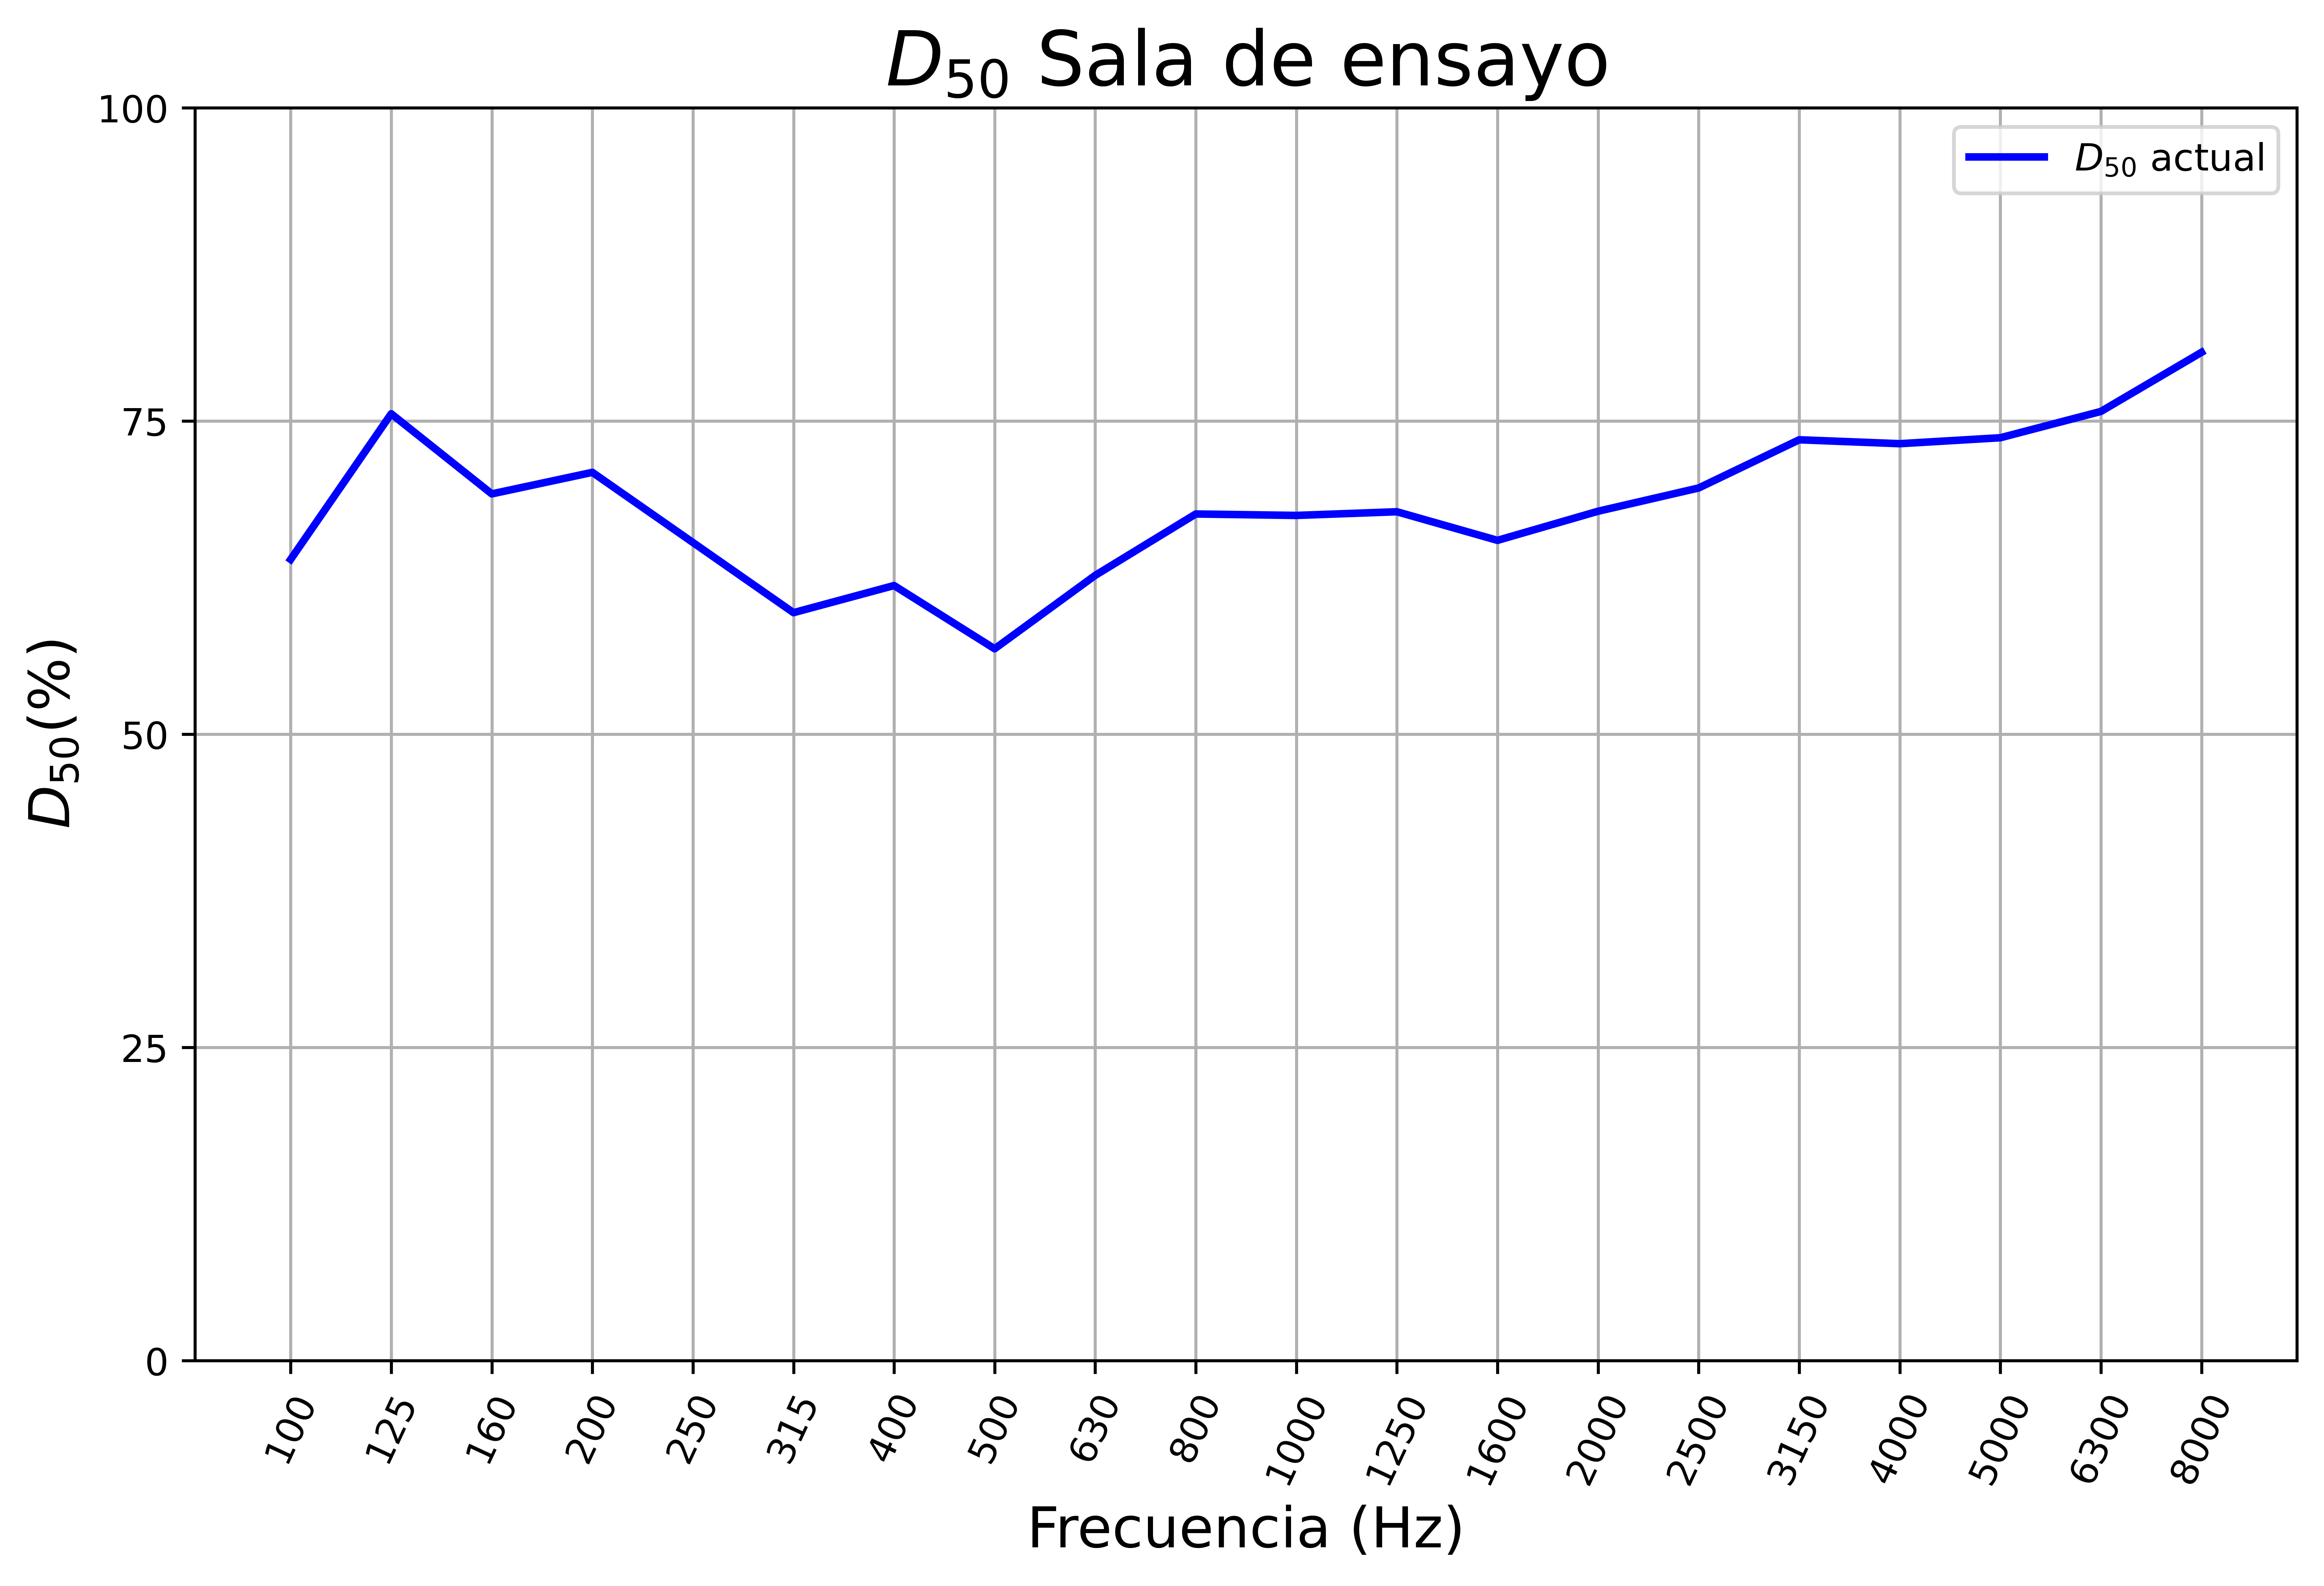
\includegraphics[width=10cm]{Imagenes/Resultados/D50_actual.png}
        \caption{$D_{50}$ de sala de ensayo}
    \end{figure}
    En la tabla \ref{tab:parametros acusticos sala ensayo} se puede observar el estado actual de la sala de ensayo determinando su $RT_{mid}$, $C_{80}$ y $D_{50}$.
    \begin{table}[H]
        \centering
        \begin{tabular}{|l|c|c|}
        \hline
        \textbf{Parámetro}& \textbf{Recomendación} & \textbf{Sala de ensayo}\\ \hline
        $RT{mid} (s)$ &  $1.3$ - $1.7$  & \textcolor{red}{$0.74$} \\ \hline
        $C_{80}$      & $-2<C_{80}<2$   & \textcolor{red}{$6.04$} \\\hline
        $D_{50}$      & $D_{50}<$ $0.5$   & \textcolor{red}{No cumple} \\\hline
        \end{tabular}
        \caption{Parámetros acústicos de la sala de ensayo y su estado}
        \label{tab:parametros acusticos sala ensayo}
    \end{table}
\subsection{Análisis modal}
Para observar el estado actual de la sala de ensayo de mejor manera, se hizo un análisis modal. En la figura ... se puede observar la distribución modal de la sala.
%insertar imagen de distribución modal
\begin{figure}[H]
    \centering
    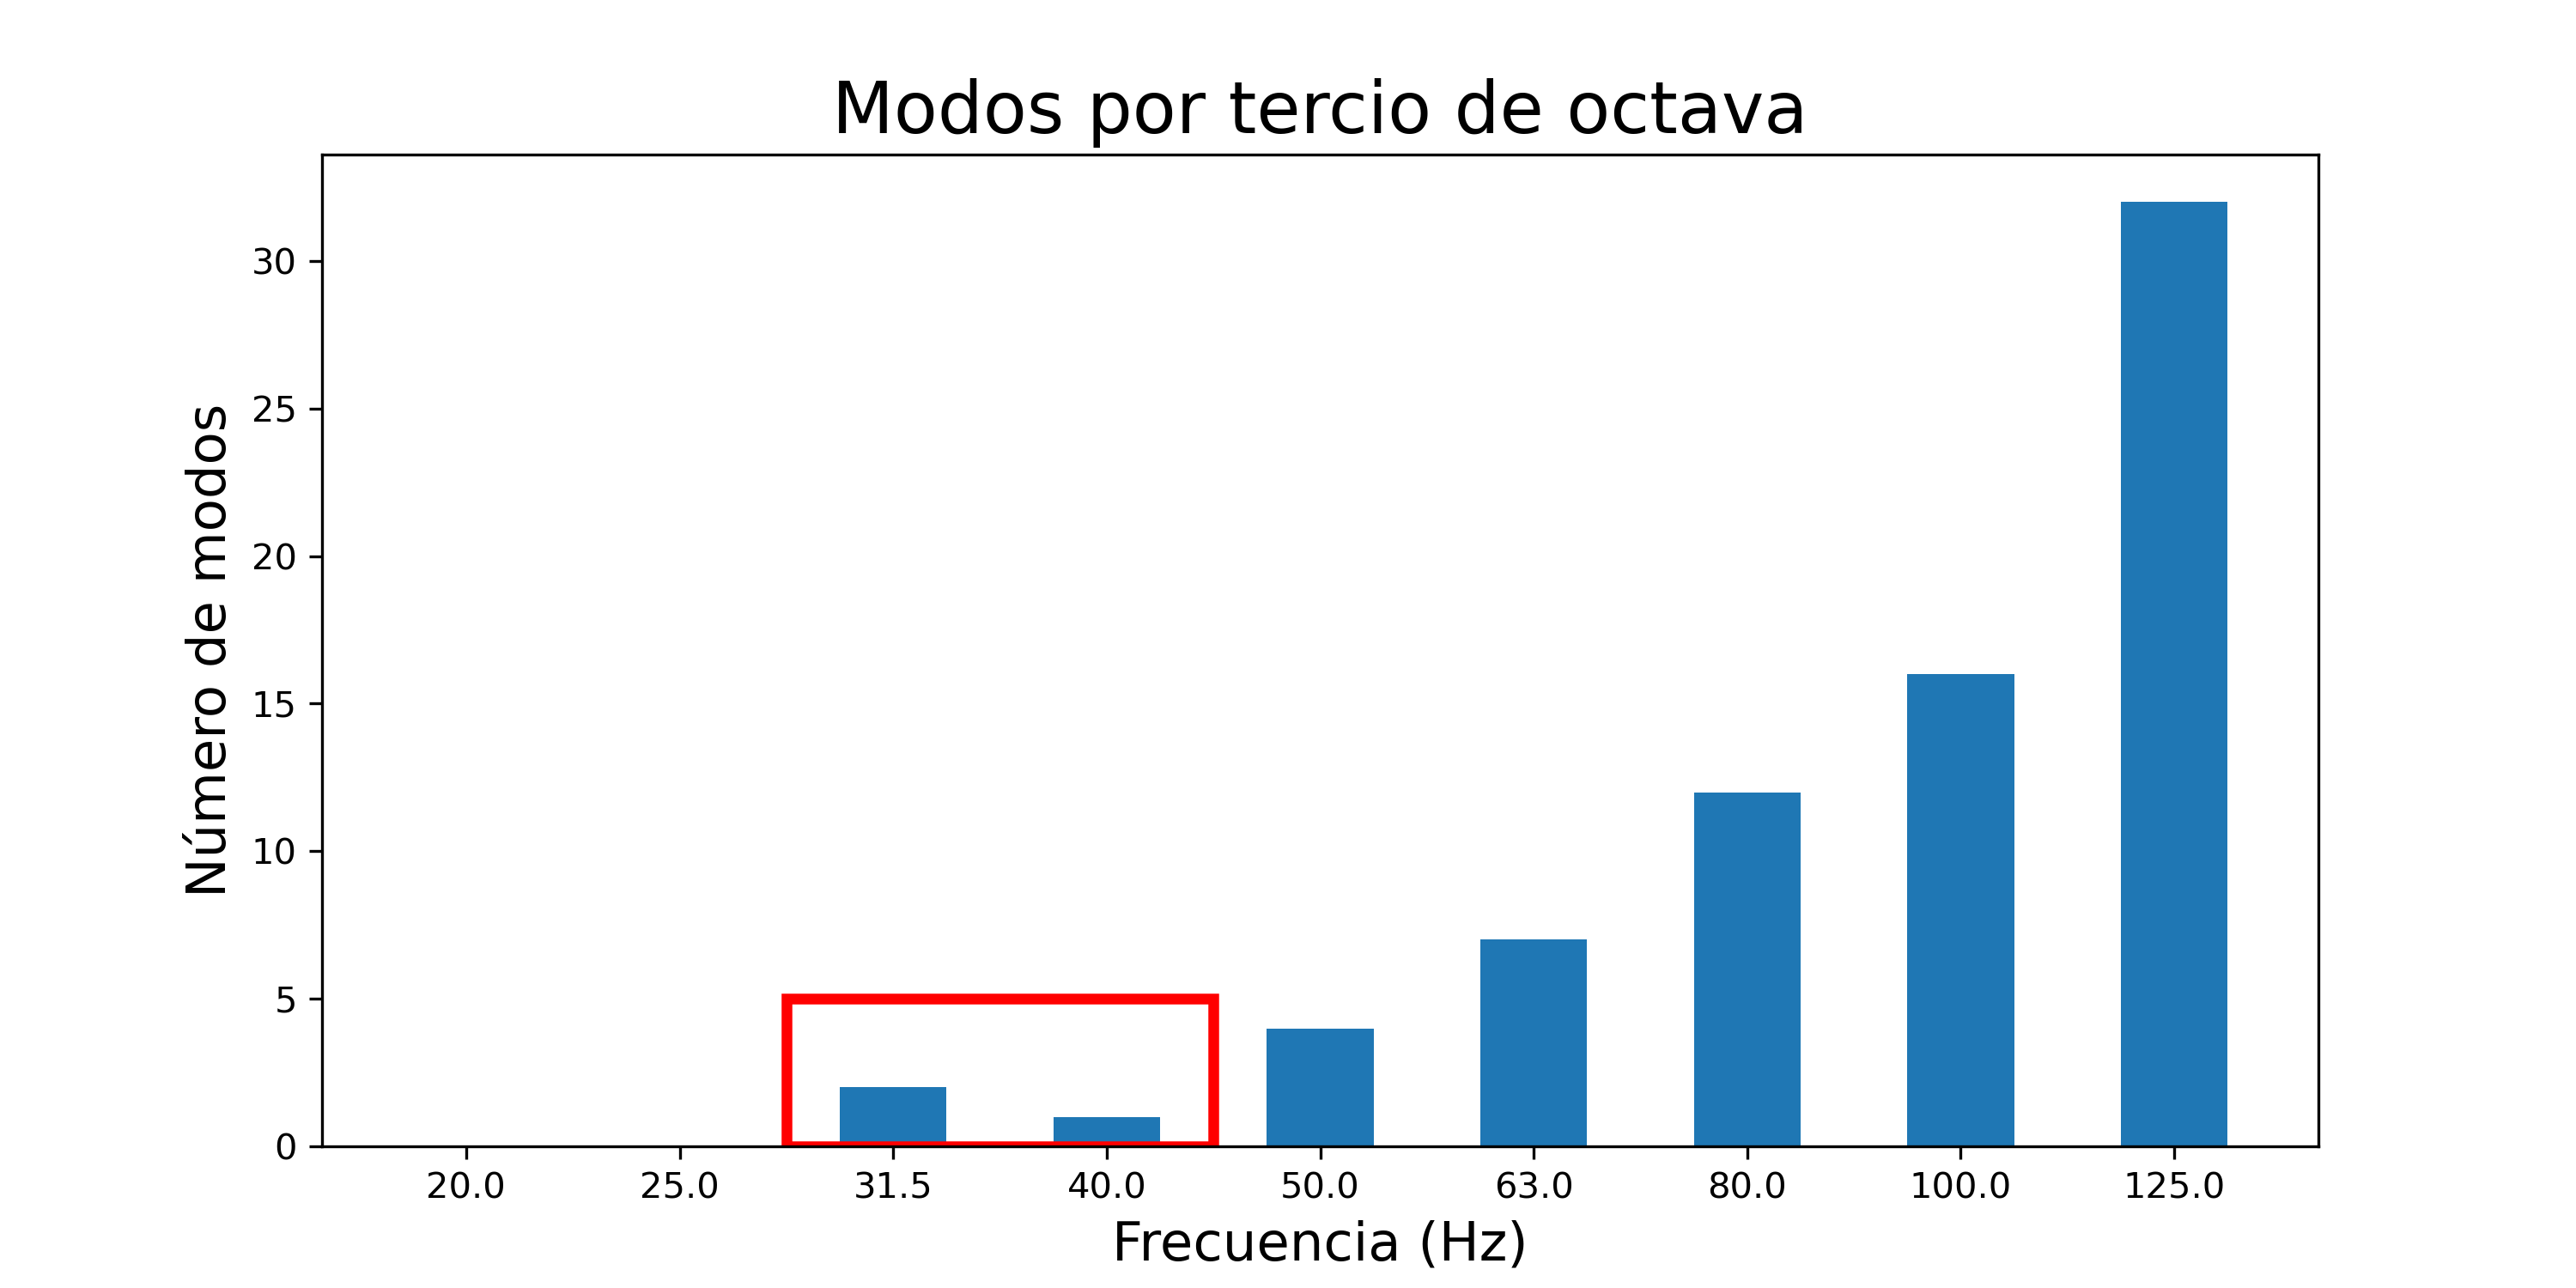
\includegraphics[width=10cm]{Imagenes/Modos/densidad modal.png}
    \caption{Distribución modal de la sala de ensayo}
    \label{fig:distribucion modal}
\end{figure}

\begin{figure}[H]
    \centering
    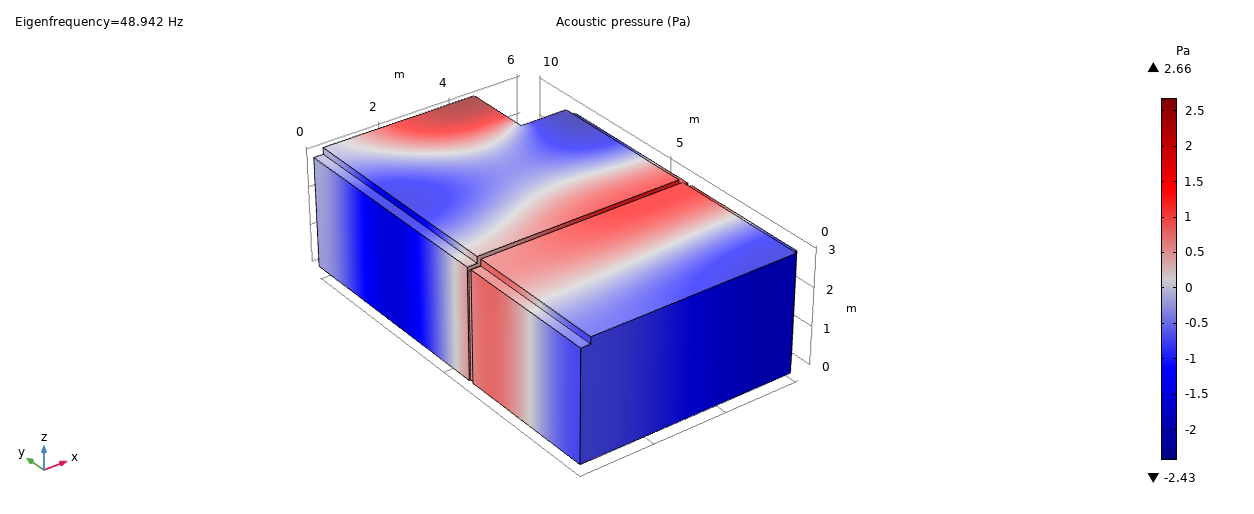
\includegraphics[width=10cm]{Imagenes/Modos/modo_48hz.png}
    \caption{Modo los 48hz}
    \label{fig:modo a los 48hz}
\end{figure}